\documentclass[a4paper]{article}
\usepackage{setspace}
\usepackage{polski}
\usepackage[utf8x]{inputenc}
\usepackage{color}
\usepackage{graphicx}
\newcommand{\HRule}{\rule{\linewidth}{0.5mm}}
\usepackage[unicode=true]{hyperref}
\usepackage{listings}

\lstset{ %
basicstyle=\footnotesize,       % the size of the fonts that are used for the code
numbers=left,                   % where to put the line\dywiz numbers
numberstyle=\footnotesize,      % the size of the fonts that are used for the line\dywiz numbers
stepnumber=2,                   % the step between two line\dywiz numbers. If it's 1, each line 
% will be numbered
numbersep=5pt,                  % how far the line\dywiz numbers are from the code
frame=single,                   % adds a~frame around the code
}

\begin{document}
\begin{titlepage}
  
  \begin{center}
    
    
    % Upper part of the page
    \includegraphics[width=0.3\textwidth]{logo.jpg}\\[1cm]    
    
    \begin{onehalfspace}
    \textsc{\LARGE Wydział Elektryczny Politechniki Warszawskiej}\\[1.5cm]
    \end{onehalfspace}
    

    
    \textsc{\Large Bazy Danych W~Systemach Rozproszonych}\\[0.5cm]
    
    
    % Title
    \HRule \\[0.4cm]
    { \huge \bfseries Badowser}\\[0.2cm]
    \HRule \\[1.5cm]
    
    % Author and supervisor
    \begin{minipage}{0.4\textwidth}
      \begin{flushleft} \large
        \emph{Autorzy:}\\
        Bartosz \textsc{Pieńkowski}
        Barnaba \textsc{Turek}
      \end{flushleft}
    \end{minipage}
    \vfill
    
    % Bottom of the page
    {\large \today}
    
  \end{center}
  
\end{titlepage}
\sloppy

\abstract{
Celem projektu jest zapoznanie się z~rozproszonym otwartym system bazodanowym CouchDB.
Projekt podzielony jest na 6 etapów, każdy z~nich odpowiada konkretnemu zagadnieniu i
związane z~nim są konkretne artefakty.
}
\section{Motyw projektu}
Projekt będzie kopiował podstawową funkcjonalność serwisów mikroblogowych (takich jak twitter).
Danymi przechowywanymi w~bazie będą więc wiadomości, posiadane przez użytkowników i~ewentualnie połączone tagami.

\section{Wstęp}
W~ramach projektu \textbf{bazy danych w~systemach rozproszonych} stworzyliśmy w~dwuosobowym zespole prosty projekt,
którego głównym celem było zapoznanie się z~problematyką rozproszonych baz danych.

\section{Co zostało wykonane}
Głównym sukcesem w~projekcie było zapoznanie się z~nowoczesną i~niezbyt popularną technologią CouchDB.
Było to o~tyle trudne, że technologia bazodanowa CouchDB jest wciąż młoda, w~związku z~czym jest słabo udokumentowana.
Do tego spotkaliśmy się z~wieloma problemami wynikającymi z~tego, że technologia jest wciąż młoda.

W~ramach zapoznawania się z~technologią CouchDB stworzyliśmy aplikację, działającą w~sposób rozproszony.
Była to aplikacja nieco przypominająca twittera pozwalająca użytkownikom dodawać wpisy.
Dodane przez użytkowników w~pisy w~czasie rzeczywistym replikowały się pomiędzy instancjami bazy danych.

Aplikacja obsługuje uwierzytelnianie użytkowników za pomocą wbudowanego systemu użytkowników CouchDB.

Pozostali klienci aplikacji otrzymują informacje o~nowych wpisach, kiedy tylko się pojawią (bez potrzeby odświeżania strony).

Ponadto aplikacja jest odporna na utratę dowolnej ilości instancji bazy, oraz na utratę połączenia pomiędzy bazami
(po odzyskaniu połączenia aplikacja automatycznie przystępuje do replikacji danych).

Dużą zaletą tej technologii jest fakt, że aplikacje są umieszczone i~serwowane z~bazy danych - nie jest potrzebny dodatkowy serwer aplikacji (np. apache, czy JBoss).


\newpage
\section{Architektura aplikacji}
\begin{figure}[bt]
  \caption{Proces renderowania strony dla klienta}
  \centering
  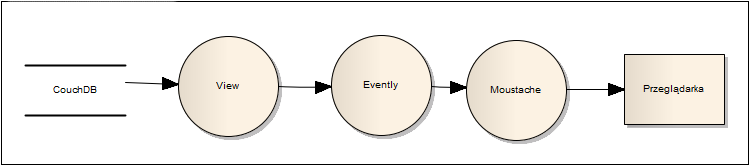
\includegraphics[width=\textwidth]{couch.png}
  \label{arch}
\end{figure}

Aplikacja została wykonana jako stos współdziałających ze sobą elementów:
\begin{itemize}
  \item CouchDB
  \item CouchApp
  \item Evently
  \item Moustache
\end{itemize}

Jej podstawą jest serwer CouchDB, który zapewnia przechowywanie informacji (zarówno o~aplikacji, jak i~informacji dodanych przez użytkowników).

Następnym elementem, jest framework CouchApp, pozwalający łatwo tworzyć aplikacje działające w~bazie danych CouchDB.
Aplikacje zbudowane przy użyciu CouchApp opierają się na technologiach HTML\dywiz 5 i~javascript (który też jest głównym językiem służącym do przetwarzania informacji w~bazie CouchDB).

Budowa aplikacji przy wykorzystaniu tej technologii polega na utworzeniu tak zwanego \emph{design document}, czyli specjalnego skryptu, opisującego aplikację.
W~tym pliku umieszczone są takie informacje, jak opis routingu aplikacji (które adresy odpowiadają jakim funkcjom w~javascripcie),
opisane są także statyczne pliki (nie zmieniające się strony, obrazki, skrypty użytkownika i~style).
Ponadto w~tym pliku umieszczone są informacje o~odczycie i~zapisie danych (czyli sposoby przygotowania danych - tzw. widoki oraz m.in. walidacje danych wprowadzonych przez użytkowników).

Użyliśmy także biblioteki evently, która pozwoliła nam na łatwą implementację tzw. push notifications, czyli wyświetlanie użytkownikom nowych postów, kiedy tylko się pojawią.

Skorzystaliśmy także z~biblioteki Moustache, która pozwala na łatwe wypełnianie szablonów stron danymi.

Współpracę wykorzystanych komponentów opisuje Rysunek \ref{arch}.

Stworzenie aplikacji w~ten sposób pozwoliło, na przechowywanie jej w~bazie. Jedną z~zalet takiego rozwiązania jest fakt, że sama aplikacja także jest replikowana.
Kolejną zaletą jest fakt, że każdy klient może posiadać własną lokalną kopię aplikacji i~z~niej korzystać (lokalna kopia aplikacji będzie miała krótsze czasy odpowiedzi na żądania klieta. 
Poza tym klient może edytować dane w~bazie, kiedy nie jest połączony z~internetem, a~kiedy się połączy mechanizm replikacji wprowadzi dokonane przez niego zmiany do głównych baz).

\section{Kod źródłowy}
Kod źródłowy dostępny jest na stronie \url{https://github.com/barnaba/badowser}.
Zastosowana struktura podziału kodu źródłowego jest wymuszona przez projekt CouchApp:
\begin{description}
  \item[evently] Przechowuje kod obsługi zdarzeń i~renderowania odpowiednich szablonów.
  \item[vendor] Przechowuje niezbędne biblioteki javascriptowe (w~tym samą bibliotekę CouchApp).
  \item[views] Przechowuje kod odpowiedzialny za zapytania.
  \item[\_attachments] Przechowuje statyczne elementy, takie jak style czy obrazki.
  \item[docs] Dokumentacja projaktu.
\end{description}
W~głównym katalogu projektu znajdują się ogólne pliki konfiguracyjne.

Ponadto część konfiguracji znajduje się w~bazie danych (np. ustawienia aplikacji).

\end{document}
